
A água potável em sua forma pura é conhecida como água destilada. Esta água é desprovida de sais minerais ou de gases.
O consumo constante de água destilada pode ser prejudicial aos seres humano devido ao fato de a ingestão diária de sais
minerais ser complementada pelos sais presentes na água mineral. Segundo resolução da Anvisa, toda água mineral no país 
que possua como objetivo ser comercializada deve ser adicionada de sais minerais. Visando seguir esta especificação e
visando não provocar um impacto na saúde dos habitantes de Acarí optou-se por adicionar sais minerais básicos à água
retirada da umidade do ar já que a falta de sais minerais na dieta dos habitantes pode levar a doenças para os mesmos,
tais como diarreia e desidratação.

Uma das propriedades mais importantes da água é o fato de ser uma substância polar, capaz de associar-se a outras substâncias 
polares ou iônicas para formar soluções aquosas. O processo de solubilização para a planta de abastecimento de água por meio
da umidade do ar pode ser realizado por um simples processo de mistura entre os sais contidos em um reservatório e a água
provinda da turbina. Portanto, será implementado um sistema de injeção e monitoramento de sais minerais à água provinda da
turbina que contará com processos mecânicos e digitais.

\begin{center}
\textbf{Mecanismos para a adição dos sais minerais}
\end{center}

  Para a adição de sais minerais na água, será implementado um mecanismo baseado em equipamentos já existentes, que injetarão
  sais minerais na água provinda da turbina. Para a realização de um processo automático de inserção de sais, será necessária 
  a utilização de um dosador automático, que varia a dosagem de uma substância de acordo com as concentrações da mesma na mistura 
  que será constantemente verificada. Existem equipamentos como o Dosimat 865, da empresa Metrohm, que possui o modo de operação
  CNT D: ao ser inserida a concentração final que se deseja de uma substância, o dosador é capaz de determinar o volume de água
  a ser adicionado para que a concentração desejada seja mantida.
  
  \begin{figure}[!htbp]
    \centering
    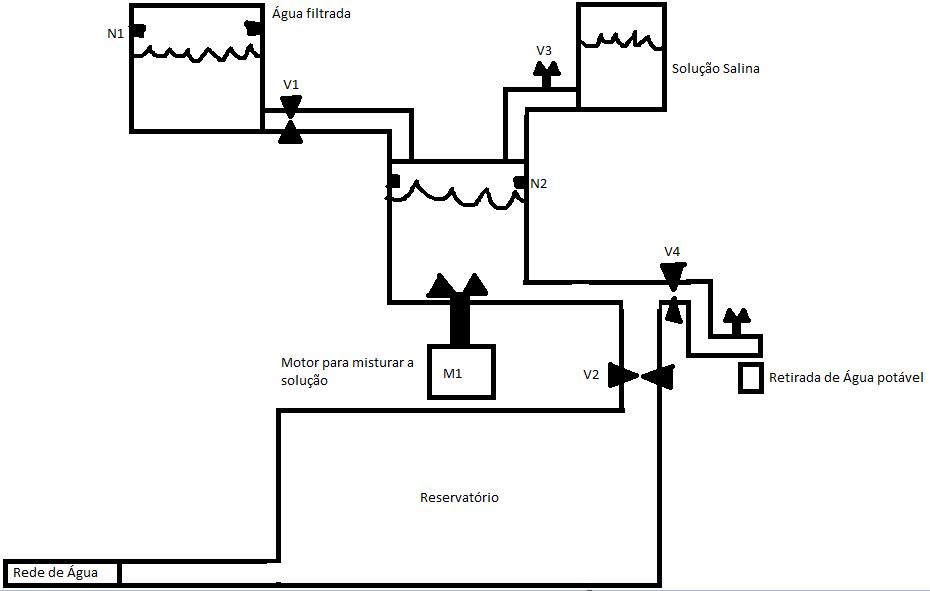
\includegraphics[scale=0.6]{editaveis/figuras/funcionamento_adicao_sais}
    \caption[Esquemático de funcionamento do controle de adição de sais]{Esquemático de funcionamento do controle de adição de sais.}
    \label{funcionamento_adicao_sais}
  \end{figure}
  \FloatBarrier
    
\begin{center}
\textbf{Funcionamento básico do sistema}
\end{center}

  \begin{itemize}
   
   \item O \textbf{sistema de controle} terá a função de enviar comandos e desta forma realizar o controle mecânico da comporta 
   que abre e fecha o tanque de armazenamento da água retirada da umidade do ar. Este sistema terá acesso direto ao aparelho
   dosador e ao sistema de sensoriamento, pois, por meio dele terá acesso às concentrações dos sais no tanque de adição. 
   Quando as concentrações de sais no tanque de adição estiverem altas, a comporta se abrirá e mais água será adicionada à 
   mistura. Por outro lado, quando as concentrações de sais estiverem baixas no tanque de adição, os comandos serão dados
   para que a comporta seja fechada. Este processo ocorrerá até que as concentrações ideais dos sais sejam atingidas.
   
   \item A \textbf{válvula de retenção} será utilizada para que a água flua apenas em um sentido, que no caso do esquemático 
   seria da esquerda para a direita. Isto impedirá que a água já adicionada de sais retorne ao tanque da água retirada da
   umidade do ar.
   
   \item O \textbf{tanque para adição de sais} será o reservatório que conterá a água adicionada de sais. Neste tanque, além
   de ocorrer a adição de sais, ocorrerá também o processo de mistura para que a solubilização dos sais na água aconteça de
   forma uniforme.
   
   \item Para o \textbf{sensoriamento} do tanque de adição de sais poderá ser utilizado um sensor de condutividade.
   Este sensor possui grande aplicabilidade a este sistema de sensoriamento, pois “A água tem um forte poder de dissociação,
   pode separar o material dissolvido em íons carregados eletronicamente. Como consequência, o material dissolvido aumenta
   bastante a condutividade da água” \cite{abilio05}.
   
  \end{itemize}
  
\begin{center}
\textbf{Misturador e dosador automático}
\end{center}

Este sistema é utilizado por empresas brasileiras para a adição de sais na água in-natura através de processos
físicos com o objetivo de produzir água tratada que é devidamente envasada e posteriormente vendida.

O princípio básico do misturador é uma máquina que provoca intensa agitação na água, dissolvendo os sais minerais. Um 
exemplo de misturador e dosador automático pode ser visto na imagem abaixo. Este equipamento é utilizado pela empresa
Amazônia- Água adicionada de sais, que produz água adicionada de sais no estado do Pará.

\begin{figure}[!htbp]
  \centering
  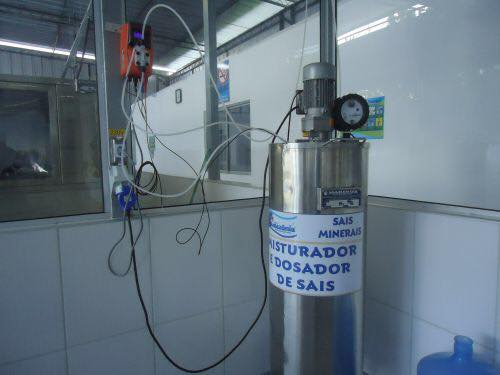
\includegraphics[scale=0.6]{editaveis/figuras/dosador_sais}
  \caption[Misturador e dosador de sais]{Misturador e dosador de sais. \footnotemark}
  \label{funcionamento_adicao_sais}
\end{figure}
\footnotetext{http://www.aguaamazonia.com/?page\_id=111}.
\FloatBarrier


\begin{center}
\textbf{Filtro adicionador de sais}
\end{center}

Existem no mercado filtros patentiados que realizam o processo de adição de sais, um bom exemplo é o ALKA WATER Biocal Ceramic 
Filter, que segundo a empresa Alka Water é um filtro que adiciona íons de cálcio, magnésio, sódio e potássio, além de ser 
aprovado pela FDA (\textit{Food and Drug Administration}).

O processo é realizado de forma passiva, necessitando apenas que a água passe pelo filtro e posteriormente seja misturada para
que a adição de sais seja realizada de maneira adequada. Um esquemático simplificado deste processo pode ser observado na imagem abaixo.

\begin{figure}[!htbp]
  \centering
  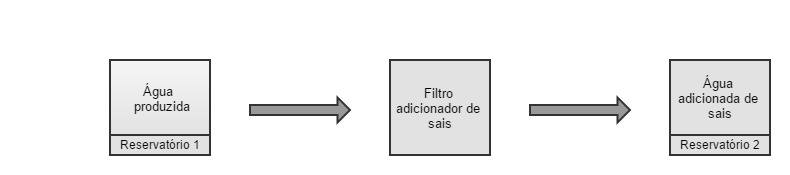
\includegraphics[scale=0.6]{editaveis/figuras/esquema_filtro_adicionador_sais}
  \caption[Esquemático do filtro adicionador de sais]{Esquemático do filtro adicionador de sais.}
  \label{esquema_filtro_adicionador_sais}
\end{figure}
\FloatBarrier


